\documentclass[10pt,a4paper]{article}
\usepackage[utf8]{inputenc}
\usepackage[spanish]{babel}
\usepackage{amsmath}
\usepackage{draftwatermark}
\SetWatermarkText{Wikipedia}
\SetWatermarkScale{5}
\SetWatermarkColor[rgb]{0.7,0,0}
\usepackage{lettrine}
\usepackage{amsfonts}
\usepackage{amssymb}
\usepackage{graphicx}
\author{Victoriano León}
\title{Los túneles de viento según la Wikipedia}
\begin{document}
\maketitle


\begin{abstract}
\lettrine{E}{n ingeniería}
, un túnel de viento o túnel aerodinámico es una herramienta de investigación desarrollada para ayudar en el estudio de los efectos del movimiento del aire alrededor de objetos sólidos. Con esta herramienta se simulan las condiciones que experimentará el objeto de la investigación en una situación real. En un túnel de viento, el objeto o modelo, permanece estacionario mientras se propulsa el paso de aire o gas alrededor de él. Se utiliza para estudiar los fenómenos que se manifiestan cuando el aire baña objetos como aviones, naves espaciales, misiles, automóviles, edificios o puentes.


\end {abstract}

\tableofcontents
\section{Historia de los túneles de viento}
El ingeniero militar inglés Benjamín Robins (1707-1751) inventó un aparato de brazo giratorio para realizar experimentos de resistencia dentro de la teoría de la aviación.
George Cayley (1773-1857), también usó un brazo giratorio para medir la resistencia y sustentación de varios álabes. Su brazo giratorio era de 5 pies de largo y logró velocidades en la punta de entre 10 y 20 pies por segundo. Armado con los datos de las pruebas del brazo, Cayley construyó un planeador pequeño que se cree que haya sido uno de los primeros vehículos más pesados que el aire que se empleó con éxito para llevar a un hombre en la historia. Sin embargo, el brazo giratorio no produce un flujo de aire que impacte las formas de la prueba a una incidencia normal. Las fuerzas centrífugas y el hecho de que el objeto está moviéndose a través de su propia estela significan que una examinación detallada del flujo de aire es difícil. Francis Herbert Wenham (1824-1908), un Miembro del Consejo de la Sociedad Aeronáutica de Gran Bretaña, arregló estos problemas, diseñando y operando el primer túnel aerodinámico en 1871.
Un túnel de viento, conocido como "tubo aerodinámico" fue diseñado y construido por Tsiolkovski en 1897.

Una vez que este descubrimiento vio la luz, datos técnicos detallados se extrajeron rápidamente. Se acredita a Wenham y a su colega Browning de muchos descubrimientos fundamentales, incluyendo la revelación de los efectos beneficiosos de una proporción del aspecto alta. Carl Rickard Nyberg usó un túnel aerodinámico al diseñar su Flugan en 1897.

En experimentos, el inglés Osborne Reynolds (1842-1912) de la Universidad de Mánchester demostraba que el patrón del flujo de aire sobre un modelo a escala sería el mismo para el vehículo real si cierto parámetro del flujo fuera el mismo en ambos casos. Este factor, ahora conocido como el Número de Reynolds, es un parámetro básico en la descripción de todas las situaciones fluido-flujo, incluyendo las formas de los patrones del flujo, la facilidad de transmisión del calor, y la presencia de la turbulencia. Esto comprende la justificación científica central para el uso de modelos en los túneles aerodinámicos al simular los fenómenos de la vida real.

Los hermanos Wright usaron un túnel aerodinámico simple en 1901 para estudiar los efectos de la corriente de aire al pasar por varias formas mientras desarrollaban a su Wright Flyer, era en parte, algo revolucionario.

El uso subsiguiente de túneles aerodinámicos fue proliferando como la ciencia aerodinámica y las disciplinas de ingeniería aeronáutica y se desarrollaron los viajes y el poder aéreo.

Los túneles aerodinámicos estaban a menudo limitados por el volumen y la velocidad de la corriente de aire que podría entregarse.

El túnel aerodinámico usado por los científicos alemanes en Peenemünde durante La Segunda Guerra Mundial es un ejemplo interesante de las dificultades asociadas con extender el rango útil de un túnel aerodinámico, donde se emplearon cuevas naturales que se aumentaron en tamaño mediante la excavación y entonces fueron selladas para guardar grandes volúmenes de aire que podría ser redireccionado a través de los túneles. Esta innovación permitió la investigación de los regímenes de alta velocidad y aceleraron la proporción y los esfuerzos de la ingeniería aeronáutica de Alemania. El primer túnel de viento supersónico fue construido en Alemania[cita requerida], con una potencia de 100.000 caballos de vapor. Después de la Segunda Guerra Mundial, fue desmantelado y trasladado a Estados Unidos.
\section{Como funciona el túnel de viento}
El aire es soplado o aspirado a través de un conducto equipado con rejillas estabilizadoras al comienzo para garantizar que el flujo se comporte de manera laminar o con obstáculos u otros objetos si se desea que se comporte de forma turbulenta. Los modelos se montan para su estudio en un equipo llamado balanza a la cual están adosados los sensores que brindan la información necesaria para calcular los coeficientes de sustentación y resistencia, necesarios para conocer si es factible o no emplear el modelo en la vida real. Además son empleados otros dispositivos para registrar la diferencia de presiones en la superficie del modelo en cuestión. Los resultados prácticos deben ser comparados con los resultados teóricos, teniendo fundamentalmente en cuenta el Número de Reynolds y el Número Mach que constituyen los criterios de validación en las pruebas con modelos a escala.
\subsection{Otras pruebas realizadas en túneles de viento}
\begin{itemize}
\item
Pueden unirse hebras a la superficie de estudio para detectar la dirección del flujo de aire y su velocidad relativa.
\item
Pueden inyectarse tintes o humo en el flujo de aire para observar el movimiento de las partículas, o sea, como se turbulizan al pasar por la superficie.
\item
Pueden insertarse sondas en puntos específicos del flujo de aire para medir la presión estática y dinámica del aire.
\end{itemize}

\subsection{Teoría de empleo de los túneles de viento}
Todos los equipos y sistemas inventados por el hombre se rigen por leyes físicas fundamentales que permiten su utilidad en la sociedad. Para un túnel aerodinámico el principio fundamental que se pone de manifiesto es el de reversibilidad del movimiento. De acuerdo a éste, en lugar de observar el movimiento de un cuerpo en su medio inmóvil, podemos observar el movimiento del medio con relación al cuerpo inmóvil. En este caso, la velocidad del flujo no perturbado en un medio reversible será igual a la velocidad del mismo cuerpo cuando el aire está inmóvil.

La posibilidad de reversibilidad del movimiento es debido a que las fuerzas aerodinámicas dependen solo del movimiento relativo del cuerpo y el aire. Cuando se proyecta cualquier tipo de avión surgen gran cantidad de problemas técnicos a resolver de forma experimental. Las aeronaves cada vez son más complejas, sus dimensiones también aumentan por lo que dificulta su experimentación a escala natural.

Todo esto, más el costo de los medios para realizar tales experimentos hace que en la aerodinámica sea muy empleado el método de modelación y simulación para la experimentación en condiciones de laboratorios, los cuales por lo general están muy lejos de las condiciones reales. Los experimentos deben simular el fenómeno de tal forma, que después sea menos complejo al proceso de modelación el cual nos permitió obtener los resultados con buen grado de aproximación a las condiciones naturales. Para lograr un proceso de modelado y simulación óptimo respecto a las condiciones reales de trabajo del objeto deben cumplirse las condiciones planteadas en la Teoría de las semejanzas.

Es necesario aclarar que para aplicaciones limitadas, la Dinámica de Fluidos Computacional (CFD, según sus siglas en inglés) puede mejorar y posiblemente reemplazar el uso de túneles de viento. Sin embargo, debe notarse que, para situaciones dónde el flujo turbulento externo está presente, el CFD no es práctico en la mayoría de los casos. Por ejemplo, las áreas que todavía son demasiado complejas para el uso de CFD están determinadas por los efectos de flujo que se observan delante y alrededor de las estructuras, puentes, terreno, etc.

La manera más eficaz de simular al flujo turbulento es mediante el uso de un túnel aerodinámico de capa límite. Los túneles aerodinámicos de capa límite son el método por excelencia de probar el flujo externo y la mayoría de los expertos están de acuerdo que esto se sostendrá hasta el futuro previsible.

Estos túneles además de ser empleados por la industria aeronáutica, son los empleados para comprobar cómo se comportarán edificaciones, puentes y todo tipo de estructuras que puedan recibir la influencia peligrosa de ráfagas de viento turbulentas.\footnote{No deben confundirse los túneles de viento con los de capa límite}

Aunque hay muchos tipos de túneles aerodinámicos, en general pueden definirse como conductos que llevan en alguna parte de su trayectoria un ventilador accionado por un motor, que se encarga de que el aire fluya de manera constante. Usualmente las palas del ventilador son diseñadas según el tipo de túnel que se construirá, de manera similar a como se hacen las de los aviones. El túnel posee una entrada convergente y una salida divergente. La parte de más interés para la experimentación es la sección de prueba o garganta, que debe, generalmente, ser transparente, para permitir la observación e incluso la filmación; en ella se instala el modelo y diferentes elementos que permiten la medición de las fuerzas que experimenta este y las condiciones del aire que atraviesa esa sección. Resulta de interés que la sección de prueba sea la de menor área, ya que, debido a la ley de conservación de la masa, genera una mayor velocidad cerca del modelo; ahorrando energía en el ventilador, ya que será capaz de generar el mismo efecto en la sección de prueba para potencias menores, además de que reduce las pérdidas por fricción en las paredes y codos del túnel.

\section{Clasificaciones de los túneles de viento}
Los túneles aerodinámicos se clasifican en función de varios aspectos los cuales son:
\subsection{Por la circulación del aire en su interior}
\begin{itemize}
\item \textbf{Abierto:}  se toma el aire directamente de la atmósfera y después de hacerlo pasar por la cámara de ensayo se devuelve nuevamente a ella.
\item \textbf{Cerrado:} el aire circula varias veces por la cámara, recuperando por medio de un difusor su energía fluida, antes de llegar de nuevo a la zona donde se encuentra instalado el difusor.

\end{itemize}

\begin{figure}[h]
\centering
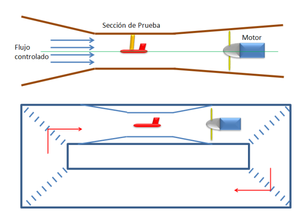
\includegraphics[scale=0.7]{tunel.png}
\label{abiertocerrado}
\caption{Aquí se ve un tunel abierto y uno cerrado}
\end{figure}
\subsection{Por la velocidad del flujo en su interior}
\begin{itemize}
\item{Subsónico}
\item{Transónico}
\item{Supersónico}
\item{Hipersónico}

\end{itemize}
\subsection{Composición general presente en los túneles de viento}
\subsubsection{Ventilador}
Produce la corriente de aire del circuito en el que se desarrolla la circulación de aire. Debe ser la velocidad adecuada para que la medición sea exacta.
\subsubsection{Cámara de ensayos}
En la que se sitúa el modelo experimental a probar. El tamaño de la cámara de ensayo es una de las características más importante de un túnel, ya que una de grandes dimensiones permite probar modelos sin gran reducción de escala con respecto al original, lo que permite mantener el índice de semejanza del número de Reynolds.
\subsubsection{Estabilizadores de corriente tras el ventilador}
Con el fin de que quede anulada la rotación comunicada por el ventilador.
\subsubsection{Difusor}
Con el objetivo de reducir la velocidad expandiendo el fluido y recuperando la presión estática, el difusor está dividido en dos partes por el ventilador. Los difusores son muy sensibles a errores de diseño, pueden crear separación de la capa límite de manera intermitente o estable que es difícil de detectar y pueden crear vibraciones en el túnel, oscilación en el ventilador y variación en la velocidad de la sección de prueba. Hay que tener en cuenta que el aire que llega al difusor no es laminar, el aire que sale de la sección de prueba no es uniforme lo que hace cada vez más difícil el trabajo del difusor.
\section{Problemas que se enfrentan con las mediciones en un túnel aerodinámico}
\subsection{Limitaciones por efecto de escala}
Estas limitaciones están dadas por la reducción del tamaño del modelo a la hora de su comprobación y análisis. Por ejemplo: un modelo de 1:4 de escala, debe ser probado a 4 veces la velocidad real. Lo cual demuestra que a medida que el modelo sea menor, mayor deberá ser la velocidad empleada en la sección de prueba, la cual puede estar limitada por la velocidad máxima del túnel con el que se cuenta. Estas limitaciones se anulan si se emplea un túnel presurizado.
\subsection{Tamaño del modelo}
Los investigadores aerodinámicos deben hallar un compromiso entre el tamaño del modelo y el del túnel. La decisión está más bien dictada por consideraciones de costo. Una vez que los números de Reynolds y Mach reales no puedan ser reproducidos, los datos experimentados son afectados por los efectos de escala, algunas veces estos últimos son despreciables. Para el caso de flujos transónicos y de baja velocidad, el efecto de escala si es considerado.
\subsection{Problemas de interferencia (fenómeno de bloqueo)}
La interferencia en la sección de prueba debido al bloqueo del flujo por el modelo es un problema que debe ser tratado con los ajustes necesarios y correcciones de los datos obtenidos. El bloqueo del flujo ocurre durante las pruebas con modelos relativamente grandes en la sección de túneles de tamaño limitado. Este bloqueo se define como el radio de la sección frontal del modelo al área de la sección de prueba. Se necesitan radios de bloqueo menores del 10\% de la sección a pesar de que muchas veces esto se excede con creces. Para las pruebas aerodinámicas, este bloqueo no debe ser mayor que el 5\%. La presencia del modelo en la sección de prueba tiene como resultado que al bloquear el flujo aumenta la presión en las paredes del túnel. Por esta razón, los túneles de sección abierta se emplean a menudo. Las correcciones por bloqueo son todavía un factor activo de investigación.
\section{Parámetros de las instalaciones de ensayo}
\footnote{para túneles subsónicos}
\begin{itemize}
\item
Bloqueo de cámara de ensayos $\frac{L^{2}}{A}$
\item
Potencia requerida $AU^{3}$
\item
Presión sobre las paredes $\rho U^{2}$
\end{itemize}
\section{fórmulas de fluidos}
\textit{Fórmula de Bernuilli}
\begin{equation}
\label{bernu}
\overbrace{{V^2 \over 2 g}}^{\mbox{cabezal de velocidad}}+\overbrace{\underbrace{\frac{P}{\gamma}}_{\mbox{cabezal de presión}} + z}^{\mbox{altura o carga piezométrica}} = \overbrace{H}^{\mbox{Cabezal o Altura hidráulica}}
\end{equation}
\vspace{2cm}


\textit{Fórmula de Bernuilli con fricción}
\begin{equation}
\label{Bernuil}
\overbrace{\frac{V_{1}^{2}}{2g}+\frac{P_{1}}{\gamma}+z_{1}+W}^{\mbox{Lado izquierdo}}=\underbrace{h_{f}+\frac{V_{2}^{2}}{2g}+\frac{P_{2}}{\gamma}+z_{2}}_{Lado derecho}
\end{equation}
\begin{figure}[h]
\centering
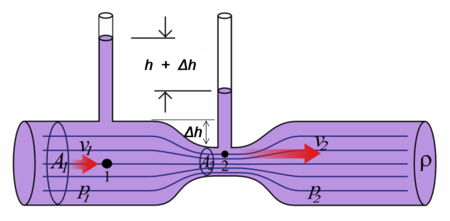
\includegraphics{bernu.png}
\caption{Flujo en tubería}
\label{tuberia}
\end{figure}
\section{Tabla de flujos y regímenes}
\begin{figure}[h]
\centering
\begin{tabular}{|c||c|c|c|c|c|} 
\hline 
&\multicolumn{5}{|c|}{Número de Reinolds}\\
\hline
\hline
$V_{a}$& Agua & GG & GX & GC & GD \\
\hline
2.5 & 2345 & 2365 & 1234 & 4570 & 65\\
\hline
3.5 & 23456 & 239785 & 1234 & 9870 & 2545\\
\hline
4.5 & 234 & 2395 & 1234 & 3270 & 255\\
\hline
5.5 & 24565 & 79865 & 1904 & 9870 & 255\\
\hline
6.5 & 2455 & 12365 & 7834 & 9870 & 5345\\
\hline
7.5 & 3445 & 2125 & 12321 & 9870 & 235\\
\hline
\end{tabular}
\label{tabla}
\caption{Tabla de referencias}
\end{figure}


\xymatrix{a\ar[r] & b
\ar[d]
\\
c
\ar[u] & d
\ar[l]}

\end{document}